\documentclass[12pt]{article}
\title{M374M Homework 1 \\
  \normalsize{\S~1.1 \#4$^1$, 5, 9$^2$, 13, 14$^3$}}
\author{Hershal Bhave (hb6279)}
\date{Due 2016-02-01}

\usepackage{macros}

\begin{document}
\maketitle

\section{\S~1.1}
\subsection{4$^1$}
  \subsubsection*{Problem}
  Assume a physical law modeling a blast wave from an atomic explosion in the
  form
  \begin{equation}
    g(t,r,\rho,E,P)=0,
  \end{equation}
  where $P$ is the ambient air pressure\footnote{$P=M L^{-1} T^{-2}$}. By
  inspection, find two independent dimensionless parameters formed from $t$,
  $r$, $\rho$, $E$, and $P$. We will name the two dimensionless parameters $\pi_1$ and
  $\pi_2$ and assume the law is equivalent to
  \begin{equation}
    f(\pi_1,\pi_2)=0.
  \end{equation}
  Does it still follow that $r$ varies like the two-fifths power of $t$?

  \subsubsection*{Remarks}
  Find the reduced form of $g(t,r,\rho,E,P)=0$ for $P\ne0$. In special case when
  $P=0$, deduce that $r=C(Et^2/\rho)^{1/5}$ as before.

  \subsubsection*{Solution}
  We will find the  $g(t,r,\rho,E,P)=0$ where $P\ne0$. Utilizing the
  mapping in \cref{fig:4-var-mappings}, we obtain the relation in
  \cref{eq:4-p-ne-step-1}.

  \begin{figure}
    \centering
    \begin{tabularx}{0.5\textwidth}{XXX}
      Variable & Dimension & Exponent \\ \hline
      $t$ & $T$ & $a$ \\
      $r$ & $L$ & $b$ \\
      $\rho$ & $ML^{-3}$ & $c$ \\
      $E$ & $ML^{2}T^{-2}$ & $d$ \\
      $P$ & $ML^{-1}T^{-2}$ & $e$ \\
    \end{tabularx}
    \caption{Variable mappings for \#4}
    \label{fig:4-var-mappings}
  \end{figure}

  \begin{equation}
    \label{eq:4-p-ne-step-1}
    \begin{aligned}
      C &= (T)^a(L)^b(ML^{-3})^c(ML^2T^{-2})^d(ML^{-1}T^{-2})^e \\
        &= M^{c+d+e}L^{b-3c+2d-e}T^{a-2d-2e} \\
    \end{aligned}
  \end{equation}

  We may now isolate the exponents for each dimension.

  \begin{equation}
    \label{eq:4-p-ne-step-2}
    \begin{aligned}
      c + d + e &= 0 \\
      b - 3c + 2d - e &= 0 \\
      a - 2d - 2e &= 0 \\
    \end{aligned}
  \end{equation}

  The resulting dimension matrix takes the form

  \begin{equation}
    \begin{pmatrix}
      0 & 0 & 1 & 1 & 1 \\
      0 & 1 & -3 & 2 & -1 \\
      1 & 0 & 0 & -2 & -2 \\
    \end{pmatrix}
  \end{equation}

  Which yields the homogenous system
  \begin{equation}
    \begin{pmatrix}
      1 & 0 & 0 & -2 & -2 \\
      0 & 1 & 0 & 5 & 2 \\
      0 & 0 & 1 & 1 & 1 \\
    \end{pmatrix} \;
    \begin{pmatrix}
      a \\ b \\ c \\ d \\ e
    \end{pmatrix}
    = 0
  \end{equation}

  Which may be solved by ``standard methods for solving linear systems.''

  \begin{equation}
    \begin{pmatrix}
      a \\ b \\ c \\ d \\ e
    \end{pmatrix}
    =
    \begin{pmatrix}
      2 \\ -5 \\ -1 \\ 1 \\ 0
    \end{pmatrix} d
    +
    \begin{pmatrix}
      2 \\ -2 \\ -1 \\ 0 \\ 1
    \end{pmatrix}
    e
  \end{equation}

  Thus we may name two linearly independent solutions which involve $P$, namely
  $d=0,\;e=1$ and $d=1,\;e=1$ (since $P\ne0$).

  \begin{multicols}{2}
    \begin{equation}
      \label{eq:4-p-ne-sol-1}
      \boxed{
        \pi_1 = t^2r^{-2}\rho^{-1}P
      }
    \end{equation}

    \begin{equation}
      \label{eq:4-p-ne-sol-2}
      \boxed{
        \pi_2 = t^4r^{-7}\rho^{-2}EP
      }
    \end{equation}
  \end{multicols}

  Furthermore, we also have a solution where $P=0$, as is the case when
  $d=1,\;e=0$.

  \begin{equation}
    \pi_3 = t^2r^{-5}\rho^{-1}E
  \end{equation}

  Solving for $r$ confirms that $r$ varies like two-fifths the power of $t$

  \begin{equation} \boxed{
      \begin{aligned}
        \pi_3 &= t^{2} r^{-5} \rho^{-1} E  \\
        r^5 &= \pi_3\left(\frac{Et^2}{\rho}\right) \\
        \implies r &= \pi_3\left(\frac{Et^2}{\rho}\right)^{1/5} \\
      \end{aligned}
    }
  \end{equation}

  \subsubsection*{Check}
  We will verify the dimensions in the case where $P\ne0$.

  \begin{equation}
    \begin{aligned}
      \pi_1 &= t^2r^{-2}\rho^{-1}P \\
      [\pi_1] &= [t]^2[r]^{-2}[\rho]^{-1}[P] \\
      0 &= T^2L^{-2}(ML^{-3})^{-1}(ML^{-1}T^{-2}) \\
      &= T^2L^{-2}M^{-1}L^{3}ML^{-1}T^{-2} \\
      &= M^{-1+1}L^{-2+3+(-1)}T^{2+(-2)} \\
      &= \cancel{M^{-1+1}}\cancel{L^{-2+3+(-1)}}\cancel{T^{2+(-2)}} \\
      \implies 0 &= 0 \quad\checkmark \\
    \end{aligned}
  \end{equation}

  \begin{equation}
    \begin{aligned}
      \pi_2 &= t^4r^{-7}\rho^{-2}EP \\
      [\pi_2] &= [t]^4[r]^{-7}[\rho]^{-2}[E][P] \\
      0 &= T^4L^{-7}(ML^{-3})^{-2}(ML^2T^{-2})(ML^{-1}T^{-2}) \\
      &= T^4L^{-7}M^{-2}L^{6}ML^2T^{-2}ML^{-1}T^{-2} \\
      &= M^{-2+1+1}L^{-7+6+2+(-1)}T^{4+(-2)+(-2)} \\
      &= \cancel{M^{-2+1+1}}\cancel{L^{-7+6+2+(-1)}}\cancel{T^{4+(-2)+(-2)}} \\
      \implies 0 &= 0 \quad\checkmark \\
    \end{aligned}
  \end{equation}

  We will verify the dimensions in the case where $P=0$.
  \begin{equation}
    \begin{aligned}
      \pi_3 &= t^{2} r^{-5} \rho^{-1} E  \\
      [\pi_3] &= [t]^{2} [r]^{-5} [\rho]^{-1} [E] \\
      0 &= T^2 L^{-5} (ML^{-3})^{-1} (ML^2T^{-2}) \\
      &= T^2 L^{-5} M^{-1}L^{3} ML^2T^{-2} \\
      &= M^{-1+1} L^{-5+3+2} T^{2+(-2)} \\
      &= \cancel{M^{-1+1}} \cancel{L^{-5+3+2}} \cancel{T^{2+(-2)}} \\
      \implies 0 &= 0 \quad\checkmark \\
    \end{aligned}
  \end{equation}

\subsection{5}
  \subsubsection*{Problem}
  A physical system is described by a law $f(E,P,A)=0$, where $E$, $P$, and $A$
  are energy, pressure, and area, respectively. Show that $PA^{3/2}/E=\text{const}$.

  \subsubsection*{Solution}
  \begin{figure}
    \centering
    \begin{tabularx}{0.5\textwidth}{XXX}
      Variable & Dimension & Exponent \\ \hline
      $E$ & $ML^2T^{-2}$ & $a$ \\
      $P$ & $ML^{-1}T^{-2}$ & $b$ \\
      $A$ & $L^2$ & $c$ \\
    \end{tabularx}
    \caption{Variable mappings for \#5}
    \label{fig:5-var-mappings}
  \end{figure}

  We may substitute the mappings in \cref{fig:5-var-mappings} into the given
  equation to define the relationship in fundamental dimensions.

  \begin{equation}
    \label{eq:5-substitution}
    \boxed{
    \begin{aligned}
      k &= \frac{PA^{3/2}}{E} \\
      [k] &= \frac{[P][A]^{3/2}}{[E]} \\
      0 &= \frac{ML^{-1}T^{-2}(L^2)^{3/2}}{ML^2T^{-2}} \\
      &= \frac{ML^2T^{-2}}{ML^2T^{-2}} \\
      \implies 0 &= 0 \\
    \end{aligned}
    }
  \end{equation}

  Thus, by dimensional analysis we can conclude that $PA^{3/2}/E=k$, where $k$
  is some dimensionless constant.

  \newpage
\subsection{9$^2$}
  \subsubsection*{Problem}
  In modeling the digestion process in the insects, it is believed that
  digestion yield rate $Y$, in mass per time, is related to the concentration
  $C$, of the limiting nutrient, the residence time $T$ in the gut, the gut
  volume $V$, and the rate of nutrient breakdown $r$, given in mass per time per
  volume. Show that for fixed $T$, $r$, $C$, the yield is positively related to
  the gut volume.

  \subsubsection*{Remarks}
  For fixed $(T,r,C)$, show that $Y$ must be proportional to
  $V$. The dimensions of concentration are $M/L^3$.

  \subsubsection*{Solution}
  \begin{figure}
    \centering
    \begin{tabularx}{0.5\textwidth}{XXX}
      Variable & Dimension & Exponent \\ \hline
      $Y$ & $MT^{-1}$ & a \\
      $C$ & $MV^{-1}$ & b \\
      $T$ & $T$ & c \\
      $V$ & $V$ & d \\
      $r$ & $MT^{-1}V^{-1}$ & e \\
    \end{tabularx}
    \caption{Variable mappings for \#9}
    \label{fig:9-var-mappings}
  \end{figure}

  The physical equation for the digestion process is given in \cref{eq:9-phy}.

  \begin{equation}
    \label{eq:9-phy}
    f(Y,C,T,V,r)
  \end{equation}

  Applying the mapping from \cref{fig:9-var-mappings} gives an equivalent
  dimensionless equation. We will use $V$ instead of $L^3$ for simplicity.

  \begin{equation}
    \label{eq:9-var}
    \begin{aligned}
      \Pi &= Y^a C^b T^c V^d r^e \\
      &= (MT^{-1})^a (MV^{-1})^b (T)^c (V)^d (MT^{-1}V)^e \\
      &= M^{a+b+e}V^{-a+c-e}T^{-b+c-e} \\
    \end{aligned}
  \end{equation}

  From \cref{eq:9-var}, we can solve the exponents such that $\Pi$ is
  dimensionless.

  \begin{equation}
    \label{eq:9-exp-eqs}
    \begin{aligned}
      a + b + e &= 0 \\
      -a + c - e &= 0 \\
      -b + d - e &= 0 \\
    \end{aligned}
  \end{equation}

  \Cref{eq:9-exp-eqs} can be rewritten in echelon form and solved by ``standard
  methods for solving linear systems''.

  \begin{equation}
    \label{eq:9-matrix}
    \begin{pmatrix}
      1 & 0 & 0 & 1 & 0 \\
      0 & 1 & 0 & -1 & 1 \\
      0 & 0 & 1 & 1 & -1 \\
    \end{pmatrix}
    \begin{pmatrix}
      a \\ b \\ c \\ d \\ e
    \end{pmatrix}
  \end{equation}

  \begin{equation}
    \label{eq:9-exp-sol}
    \implies
    \begin{pmatrix}
      a \\ b \\ c \\ d \\ e
    \end{pmatrix}
    =
    \begin{pmatrix}
      -1 \\ 1 \\ -1 \\ 1 \\ 0
    \end{pmatrix}d +
    \begin{pmatrix}
      0 \\ -1 \\ 1 \\ 0 \\ 1
    \end{pmatrix}e
  \end{equation}

  From \cref{eq:9-exp-sol} we may now show that $Y$ must be proportional to $V$
  in two linearly independent solutions. The two cases in particular are when
  $d=1, e=0$; $d=1, e=1$. We must utilize $d$ in each case to maintain $Y$'s
  proportionality to $V$.

  \begin{multicols}{2}
    \begin{equation}
      \label{eq:9-sol-1}
      \boxed{
      \begin{aligned}
        \Pi &= Y^{-1} C^{1} T^{-1} V^1 r^0 \\
        \implies Y &= \Pi\;\frac{CV}{T} \\
      \end{aligned}
      }
    \end{equation}

    \begin{equation}
      \label{eq:9-sol-2}
      \boxed{
      \begin{aligned}
        \Pi &= Y^{-1} C^{0} T^{0} V^1 r^0 \\
        \implies Y &= \Pi\; Vr \\
      \end{aligned}
      }
    \end{equation}
  \end{multicols}

  \subsubsection*{Check}
  We will verify that the dimensions in \cref{eq:9-sol-1} are correct.

  \begin{equation}
    \begin{aligned}
      [Y] &= \frac{[C][V]}{[T]} \\
      MT^{-1} &= \frac{MV^{-1}V}{T} \\
      MT^{-1} &= MV^{-1}VT^{-1} \\
      MT^{-1} &= M\cancel{V^{-1}}\cancel{V}T^{-1} \\
      \implies MT^{-1} &= MT^{-1} \quad\checkmark \\
    \end{aligned}
  \end{equation}

  We will verify that the dimensions in \cref{eq:9-sol-2} are correct.

  \begin{equation}
    \begin{aligned}
      [Y] &= [V] [r] \\
      MT^{-1} &= V MT^{-1}V^{-1} \\
      MT^{-1} &= \cancel{V} MT^{-1} \cancel{V^{-1}} \\
      \implies MT^{-1} &= MT^{-1} \quad\checkmark \\
    \end{aligned}
  \end{equation}

  \newpage
  \subsection{13}
  \subsubsection*{Problem}
  Imagine an experiment where we set up a line of dominos with spacing $d$
  between them. Further, we assume a typical domino has height $h$ and thickness
  $\tau$. We seek a formula that relates these quantities, the gravitational
  constant $g$, and the velocity $v$.

  \begin{enumerate}
  \item Use dimensional analysis to show
    that
    \begin{equation}
      \label{eq:13-1-question}
      v=\sqrt{gh}\; F\left(\frac{d}{h},\frac{\tau}{h}\right).
    \end{equation}
    Assume $\tau/h$ is very small and can be neglected. What does the law become?
  \item Experiments have been performed that show the graph of $v/\sqrt{gh}$ vs.
    $d/h$ is approximately constant, $1.5$, for $d/h$ varying over the range $0$
    to $0.8$. Using $h=0.05$ meters, what is the velocity of the toppling dominos?
  \end{enumerate}

  \subsubsection*{Solution}
  \begin{enumerate}
  \item We will first prove \cref{eq:13-1-question}. $F$ is some dimensionless
    quantity. We will verify that the dimensions match up

    \begin{equation}
      \begin{aligned}
        [v] &= [g]^{1/2}[h]^{1/2} \\
        LT^{-1} &= LT^{-2}T \\
        \implies LT^{-1} &= LT^{-1}. \quad \checkmark \\
      \end{aligned}
    \end{equation}

    Assuming that $\tau/h$ is small, the law becomes
    \begin{equation} \boxed {
        \label{eq:13-1-new-law}
        v=\sqrt{gh}\; F\left(\frac{d}{h}\right).
      }
    \end{equation}

  \item Since $d/h$ is approximately constant, we can model the quantity by the
    given constant ($d/h=1.5$) in \cref{eq:13-1-new-law}.

    \begin{equation} \boxed{
        \begin{aligned}
          v &= \sqrt{gh}(1.5) \\
          &= \sqrt{9.8\cdot0.05}(1.5) \\
          \implies v &= 1.05 \text{ m/s}
        \end{aligned}
      }
    \end{equation}
  \end{enumerate}

  \subsubsection*{Check}
  \todo

\subsection{14$^3$}
  \subsubsection*{Problem}
  A perfect gas in equilibrium has specific energy $E$ (energy per mass),
  temperature $T$, and Boltzmann constant $k$ (specific energy per degress).
  Derive a functional relationship of the form $E=f(T,k)$.

  \subsubsection*{Remarks}
  Assuming a law $F(E,T,k)=0$, derive an equivalent reduce law and show that
  $E=Tck$ for some constant $c$.

  \subsubsection*{Solution}

  \begin{figure}
    \centering
    \begin{tabularx}{0.5\textwidth}{XXX}
      Variable & Dimension & Exponent \\ \hline
      $E$ & $L^2T^{-2}$ & a \\
      $T$ & $\Theta$ & b \\
      $k$ & $L^2T^{-2}\Theta^{-1}$ & c \\
    \end{tabularx}
    \caption{Variable mappings for \#14}
    \label{fig:14-var-mappings}
  \end{figure}

  Given the physical relationship $F(E,T,k)=0$ and the variable mappings in
  \cref{fig:14-var-mappings}, we may derive an equivalent dimensionless physical
  relationship between $E$, $T$, and $k$.

  \begin{equation}
    \begin{aligned}
      \pi &= E^aT^bk^c \\
      &= (L^2T^{-2})^a (\Theta)^{b} (L^2T^{-2}\Theta^{-1})^c = 1\\
    \end{aligned}
  \end{equation}

  By inspection we can clearly see that $a=1$, $b=-1$, and $c=-1$. Thus

  \begin{equation}
    \pi = \frac{E}{Tk}
  \end{equation}

  This makes the equivalent dimensionless physical relationship

  \begin{equation}
    g\left(\frac{E}{Tk}\right) = 0
  \end{equation}

  Which means that the physical law must take the form

  \begin{equation}
    \frac{E}{Tk} = c
  \end{equation}

  Solving for $E$ gives us

  \begin{equation}
    \boxed{
      \begin{aligned}
        E &= Tck \\
        E &= f(T,k) \\
      \end{aligned}
    }
  \end{equation}

  \subsubsection*{Check}
  Utilizing the dimensions from the mapping in \cref{fig:14-var-mappings}, we
  may verify by inspection.

  \begin{equation}
    \begin{aligned}
      E &= Tck \\
      [E] &= [T][k] \\
      L^2T^{-2} &= L^2T^{-2}\Theta^{-1} \Theta \\
       &= L^2T^{-2} \cancel{\Theta^{-1}} \cancel{\Theta} \\
      \implies L^2T^{-2} &= L^2T^{-2} \quad\checkmark \\
    \end{aligned}
  \end{equation}


\section{Programming Minilab}
A model for an ideal pendulum released from rest is

\begin{equation}
  \label{eq:minilab-pendulum-model}
   \left\{
  \begin{aligned}
    &\ell\ddot{\theta}+g\sin\theta = 0, \quad &t &\ge0 \\
    &\dot{\theta} = 0, \quad &t &= 0 \\
    &\theta = \theta_0, \quad &t &= 0. \\
  \end{aligned}\right.
\end{equation}

Here $\theta$ is the pendulum angle, $\ell$ is the pendulum length, $g$ is the
gravitational acceleration constant, $t$ is time, and over-dots denote time
derivatives. A dimensional analysis of \cref{eq:minilab-pendulum-model} reveals
that the general solution can be written in the form

\begin{equation}
  \label{eq:minilab-general-solution}
  \theta = \tilde{f}(t\sqrt{g/\ell}, \;\theta_0)
\end{equation}
for some function $\tilde{f}$. Here we investigate various consequences of
\cref{eq:minilab-general-solution}. We will use meters and seconds as our units
for length and time, respectively.

\subsection{}
  \label{sec:minilab-part-1}
  \subsubsection*{Problem}
  For the initial conditions $\theta_0=3\pi/8$ and interval $t\in[0,2.5]$,
  superimpose plots of $\theta$ versus $t$ for different values of $g$ and $\ell$,
  say, $(g,\ell)=(10, 0.25), (10, 0.5), (10, 1)$. Based on the general solution
  $\theta = f(t,g,\ell,\theta_0)$, briefly explain why different values of $g$ and
  $\ell$ produce different curves.

  \subsubsection*{Solution}
  Reference \cref{fig:2-1-solution}. It seems that different values of $g$ and
  $\ell$ produce the same curve with different scaling. Based on the general
  solution, $\theta$ is inversely proportional to the square root of $\ell$.
  Thus when $\ell$ varies between $0.25$ to $1$, the curve halves in frequency.

  \begin{figure}
    \centering
    \scalebox{0.8}{\huge% Title: glps_renderer figure
% Creator: GL2PS 1.3.9, (C) 1999-2015 C. Geuzaine
% For: Octave
% CreationDate: Sun Jan 31 20:25:04 2016
\setlength{\unitlength}{1pt}
\begin{picture}(0,0)
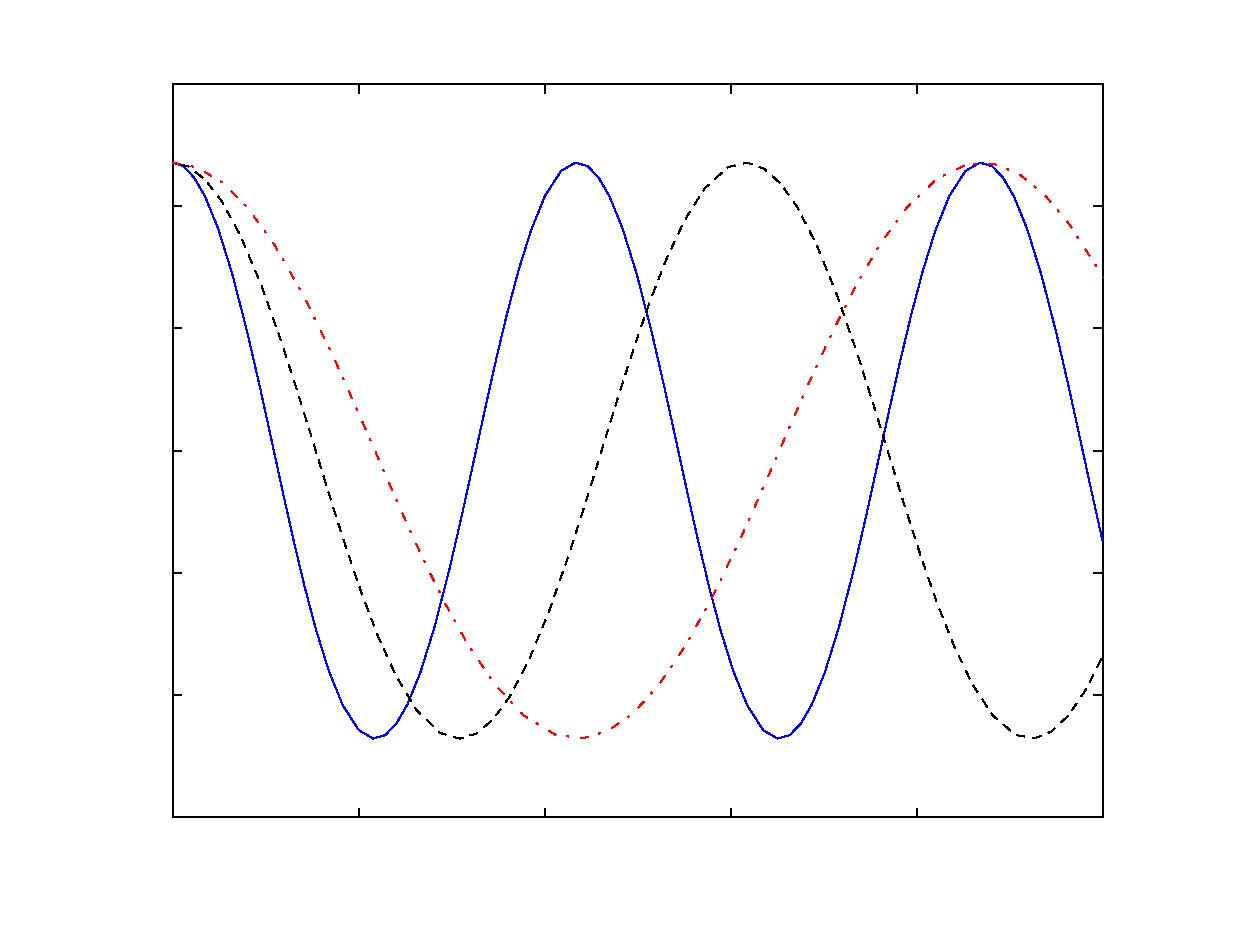
\includegraphics{prog1_fig1-inc}
\end{picture}%
\begin{picture}(576,432)(0,0)
\fontsize{10}{0}
\selectfont\put(74.88,42.5189){\makebox(0,0)[t]{\textcolor[rgb]{0,0,0}{{0}}}}
\fontsize{10}{0}
\selectfont\put(164.16,42.5189){\makebox(0,0)[t]{\textcolor[rgb]{0,0,0}{{0.5}}}}
\fontsize{10}{0}
\selectfont\put(253.44,42.5189){\makebox(0,0)[t]{\textcolor[rgb]{0,0,0}{{1}}}}
\fontsize{10}{0}
\selectfont\put(342.72,42.5189){\makebox(0,0)[t]{\textcolor[rgb]{0,0,0}{{1.5}}}}
\fontsize{10}{0}
\selectfont\put(432,42.5189){\makebox(0,0)[t]{\textcolor[rgb]{0,0,0}{{2}}}}
\fontsize{10}{0}
\selectfont\put(521.28,42.5189){\makebox(0,0)[t]{\textcolor[rgb]{0,0,0}{{2.5}}}}
\fontsize{10}{0}
\selectfont\put(69.8755,47.52){\makebox(0,0)[r]{\textcolor[rgb]{0,0,0}{{-1.5}}}}
\fontsize{10}{0}
\selectfont\put(69.8755,106.2){\makebox(0,0)[r]{\textcolor[rgb]{0,0,0}{{-1}}}}
\fontsize{10}{0}
\selectfont\put(69.8755,164.88){\makebox(0,0)[r]{\textcolor[rgb]{0,0,0}{{-0.5}}}}
\fontsize{10}{0}
\selectfont\put(69.8755,223.56){\makebox(0,0)[r]{\textcolor[rgb]{0,0,0}{{0}}}}
\fontsize{10}{0}
\selectfont\put(69.8755,282.24){\makebox(0,0)[r]{\textcolor[rgb]{0,0,0}{{0.5}}}}
\fontsize{10}{0}
\selectfont\put(69.8755,340.92){\makebox(0,0)[r]{\textcolor[rgb]{0,0,0}{{1}}}}
\fontsize{10}{0}
\selectfont\put(69.8755,399.6){\makebox(0,0)[r]{\textcolor[rgb]{0,0,0}{{1.5}}}}
\fontsize{10}{0}
\selectfont\put(298.08,31.5189){\makebox(0,0)[t]{\textcolor[rgb]{0,0,0}{{t}}}}
\fontsize{10}{0}
\selectfont\put(43.8755,223.56){\rotatebox{90}{\makebox(0,0)[b]{\textcolor[rgb]{0,0,0}{{$\theta$}}}}}
\fontsize{10}{0}
\selectfont\put(298.08,409.6){\makebox(0,0)[b]{\textcolor[rgb]{0,0,0}{{L=0.25 (blue,solid), 0.5 (black,dash), 1 (red,dashdot)}}}}
\end{picture}
}
    \caption{$\theta$ vs $t$ for varying values of $\ell$}
    \label{fig:2-1-solution}
  \end{figure}

\subsection{}
  \label{sec:minilab-part-2}
  \subsubsection*{Problem}
  Repeat \cref{sec:minilab-part-1} but now plot $\theta$ vs $t\sqrt{g/\ell}$.
  Based on the form of the solution in \cref{eq:minilab-general-solution},
  briefly explain why different values of $g$ and $\ell$ produce the same curve
  (or portion thereof). If $\theta_0$ were changed in addition to $g$ and
  $\ell$, would we still get this same curve?

  \subsubsection*{Solution}
  Reference \cref{fig:2-2-solution}. Dimensional analysis of the quantity
  $t\sqrt{g/\ell}$ reveals that $t\sqrt{g/\ell}$ is dimensionless. This means
  that the plot of $\theta$ vs. $t\sqrt{g/\ell}$ effectively rescales the
  dimensions in \cref{fig:2-1-solution} to produce \cref{fig:2-2-solution}.
  Since the pendulum with the smallest length has the fastest frequency, its
  curve is the longest. Furthermore, changing $\theta_0$ in addition to $g$ and
  $\ell$ should produce the same curve since angles are dimensionless.

  \begin{figure}
    \centering
    \scalebox{0.8}{\huge% Title: glps_renderer figure
% Creator: GL2PS 1.3.9, (C) 1999-2015 C. Geuzaine
% For: Octave
% CreationDate: Sun Jan 31 20:53:05 2016
\setlength{\unitlength}{1pt}
\begin{picture}(0,0)
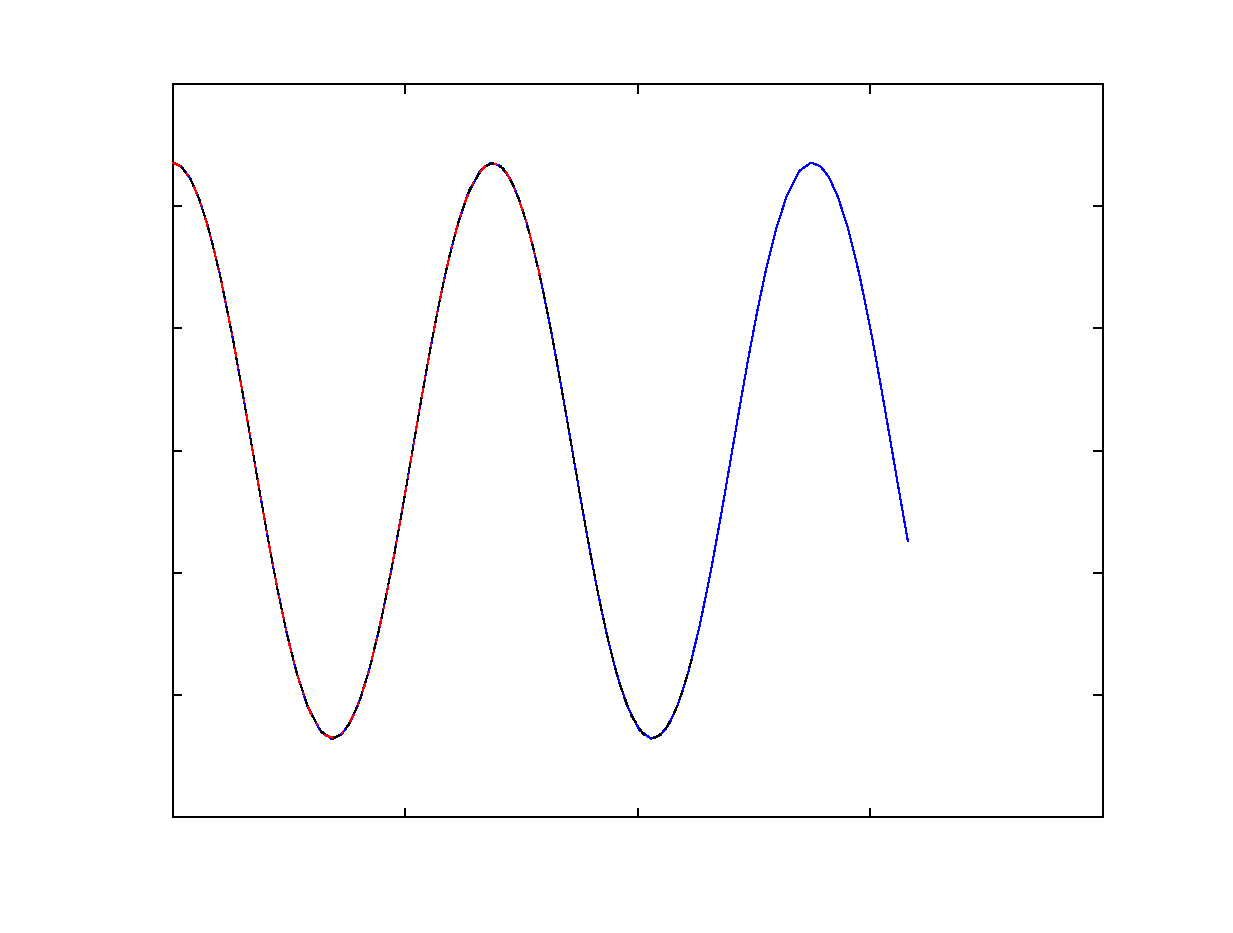
\includegraphics{prog1_fig2-inc}
\end{picture}%
\begin{picture}(576,432)(0,0)
\fontsize{10}{0}
\selectfont\put(74.88,42.5189){\makebox(0,0)[t]{\textcolor[rgb]{0,0,0}{{0}}}}
\fontsize{10}{0}
\selectfont\put(186.48,42.5189){\makebox(0,0)[t]{\textcolor[rgb]{0,0,0}{{5}}}}
\fontsize{10}{0}
\selectfont\put(298.08,42.5189){\makebox(0,0)[t]{\textcolor[rgb]{0,0,0}{{10}}}}
\fontsize{10}{0}
\selectfont\put(409.68,42.5189){\makebox(0,0)[t]{\textcolor[rgb]{0,0,0}{{15}}}}
\fontsize{10}{0}
\selectfont\put(521.28,42.5189){\makebox(0,0)[t]{\textcolor[rgb]{0,0,0}{{20}}}}
\fontsize{10}{0}
\selectfont\put(69.8755,47.52){\makebox(0,0)[r]{\textcolor[rgb]{0,0,0}{{-1.5}}}}
\fontsize{10}{0}
\selectfont\put(69.8755,106.2){\makebox(0,0)[r]{\textcolor[rgb]{0,0,0}{{-1}}}}
\fontsize{10}{0}
\selectfont\put(69.8755,164.88){\makebox(0,0)[r]{\textcolor[rgb]{0,0,0}{{-0.5}}}}
\fontsize{10}{0}
\selectfont\put(69.8755,223.56){\makebox(0,0)[r]{\textcolor[rgb]{0,0,0}{{0}}}}
\fontsize{10}{0}
\selectfont\put(69.8755,282.24){\makebox(0,0)[r]{\textcolor[rgb]{0,0,0}{{0.5}}}}
\fontsize{10}{0}
\selectfont\put(69.8755,340.92){\makebox(0,0)[r]{\textcolor[rgb]{0,0,0}{{1}}}}
\fontsize{10}{0}
\selectfont\put(69.8755,399.6){\makebox(0,0)[r]{\textcolor[rgb]{0,0,0}{{1.5}}}}
\fontsize{10}{0}
\selectfont\put(298.08,31.5189){\makebox(0,0)[t]{\textcolor[rgb]{0,0,0}{{$t\sqrt{g/\ell}$}}}}
\fontsize{10}{0}
\selectfont\put(43.8755,223.56){\rotatebox{90}{\makebox(0,0)[b]{\textcolor[rgb]{0,0,0}{{$\theta$}}}}}
\fontsize{10}{0}
\selectfont\put(298.08,409.6){\makebox(0,0)[b]{\textcolor[rgb]{0,0,0}{{L=0.25 (blue,solid), 0.5 (black,dash), 1 (red,dashdot)}}}}
\end{picture}
}
    \caption{$\theta$ vs $t\sqrt{g/\ell}$ for varying values of $\ell$}
    \label{fig:2-2-solution}
  \end{figure}

\subsection{}
  \subsubsection*{Problem}
  Let $T$ be the period of the pendulum motion for given $\theta_0$, $g$, $\ell$.
  Using the form of the solution in \cref{eq:minilab-general-solution}, show

  \begin{equation}
    \label{eq:2-3-prob}
    T=\sqrt{\ell/g}\;h(\theta_0)
  \end{equation}

  for some function $h$. Does this agree with the
  observations in \cref{sec:minilab-part-1}? Specifically, for fixed $\theta_0$
  and $g$, does $T$ increase by a factor of two when $\ell$ is increased by a
  factor of four?

  \subsubsection*{Solution}

  Since $\theta$ in \cref{eq:minilab-general-solution} is dimensionless, we may
  utilize the Pi theorem to obtain a relation for $h(\theta_0)$.

  \begin{equation}
    \begin{aligned}
      \theta &= \tilde{f}(t\sqrt{g/\ell},\;\theta_0) \\
      &= \tilde{f}(\pi_1,\;\pi_2) \\
      0 &= F(\pi_1,\;\pi_2) \\
      \pi_1 &= h(\pi_2) \\
      \implies t\sqrt{g/\ell} &= h(\theta_0) \\
    \end{aligned}
  \end{equation}

  Since $t\sqrt{g/\ell}$ is dimensionless, we may confirm that $h(\theta_0)$ is
  also dimensionless. Through dimensional analysis we may also confirm that the
  dimensions in \cref{eq:2-3-prob} agree.

  \begin{equation}
    \begin{aligned}
      T &= \sqrt{\ell/g}\;h(\theta_0) \\
      [T] &= [\ell]^{-1/2}[g]^{1/2} \\
      T &= L^{-1/2}(LT^2)^{1/2} \\
      &= L^{-1/2}L^{1/2}T \\
      &= \cancel{L^{-1/2}}\cancel{L^{1/2}}T \\
      T &= T \quad\checkmark
    \end{aligned}
  \end{equation}

  This agrees with the observations in \cref{sec:minilab-part-1}; since $T$
  varies in relation to $\ell$ by square root, quadrupling $\ell$ doubles $T$.

\end{document}
